\documentclass[12pt, titlepage]{article}

\usepackage{booktabs}
\usepackage{tabularx}
\usepackage{hyperref}
\usepackage{enumerate}
\usepackage{graphicx}
\usepackage{setspace}
\usepackage{float} 
\usepackage[numbers]{natbib}
\bibliographystyle{IEEEtranN}
\renewcommand{\bibsection}{}

\newcolumntype{Y}{>{\centering\arraybackslash}X}
\title{\textbf{SE 3XA3: Software Requirements Specification} \\
    \large{Tetris Tussle \\ Group 2}
}
\author{
    Nicholas Lobo \\ lobon3 \\ 400179304 \and
	Matthew Paulin \\ paulinm \\ 400187147 \and
	David Carrie \\ carriedd \\ 000661652 \and
}
\date{\today}



\begin{document}

\maketitle

\pagenumbering{roman}
\tableofcontents
\listoftables
\listoffigures

\begin{table}[!ht]
\caption{\bf Revision History}
\begin{tabularx}{\textwidth}{p{3cm}p{2cm}X}
\toprule {\bf Date} & {\bf Version} & {\bf Notes}\\
\midrule
February 7 2021 & 1.0 & Section 1, Non-Functional Requirements\\
February 10 2021 & 1.1 & Section 2\\
February 11 2021 & 1.2 & Section 4, Functional Requirements \\
February 12 2021 & 1.3 & Corrected grammar and added detail\\
\bottomrule
\end{tabularx}
\end{table}

\newpage
\pagenumbering{arabic}

\section{Project Drivers}
\subsection{The Purpose of the Project}
With the recent emergence of large scale triple A games with advanced features flooding the market there has been an absence of puzzle games that require quick decision making and careful planning. It was decided to put a spin on a simple but beloved classic to fill that void. Tetris took the world by storm in the 1980’s becoming the first hit game ever created by selling over 202 million copies. The aim of this project is to take a bare bones version of this game and update it to better suit the modern standards of gaming through updated visuals and player versus player (PvP) interaction.
\subsection{The Stakeholders}
\subsubsection{The Client}
The clients for this system are Dr. Asghar Bokhari, the professor for 3XA3 as well as the teaching assistants for this course. These clients are responsible for monitoring the development of the product and ensuring it meets their given criteria. They can also offer clarification for any ambiguities about the project. Lastly, they will determine the degree to which the requirements in this document are met by the final product.
\subsubsection{The Customers}
The customers include anyone who will play Tetris Tussle. This includes people of all ages who own or have access to a computer. They must also have a stable internet connection to access the game as well as a modern web browser. The customers will use the software as a form of entertainment and to compete with people around the globe.
\subsubsection{Other Stakeholders}
Any current or future developers of this project are also stakeholders.
\subsection{Mandated Constraints}
\begin{itemize}
    \item The product must be completed by the week of April 12\textsuperscript{th}.
    \item The product must be playable on Windows 10, Mac OSX, and Linux.
    \item The product shall support automated testing.
    \item The product must be free to play.
    \item The product must remain open source.
    \item Development costs shall not exceed \$0.
    \item The project must be a redevelopment of an open source project.
    \item The project shall contain some graphical or gameplay improvements compared to the original.
\end{itemize}
\subsection{Naming Conventions and Terminology}
\textbf{Tetromino}: A Tetromino is the geometric shape used in Tetris. It is composed of four squares connected at their edges to form 7 different shapes.
\begin{itemize}
    \item \textbf{Active Tetromino:} A Tetromino that can be moved by the player.  
    \item \textbf{Held Tetromino:} A Tetromino that is saved and can be used at another time by the player
    \item \textbf{Dead Tetromino:} Is when the bottom of an Active Tetromino hits the top of a Dead Tetromino or the end of the board.
\end{itemize}
\subsection{Relevant Facts and Assumptions}
\begin{itemize}
    \item Users can read English at an intermediate level.
    \item Users can operate a computer.
    \item Users can navigate the internet with a modern web browser.
    \item Users will have a system with at least 2GB of RAM and a processor clock speed of at least 1GHz.
\end{itemize}

\section{Functional Requirements}
\subsection{The Scope of the Work and the Product}
The scope of work is the redevelopment of the open source project located at \url{https://github.com/dionyziz/canvas-tetris}. The project scope contains additional elements as well as redeveloping and implementing the core game of Tetris. These additional elements are: a user interface including a game menu, a scoring and leader board system, and the ability to play a 2 player multiplayer game. We will only be providing the software and system to enable users to access the features above through modern web browsers with JavaScript enabled and over an internet connection.

\subsubsection{The Context of the Work}
\begin{figure}[H]
    \centering
    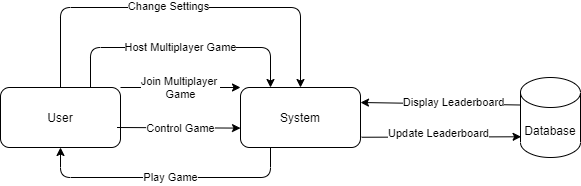
\includegraphics[width=5in]{WorkContext.png} 
    \caption{Work Context Diagram}
    \label{fig:work_context}
\end{figure}
\subsubsection{Work Partitioning}
\begin{table}[!ht]
\centering
\caption{\bf Work Partitioning}
\begin{tabularx}{\textwidth}{@{}|Y|Y|Y|Y|@{}}
\hline
Event Number & Event Name & Input & Output \\
\hline
1 & View Leader board & Mouse & Leader Board \\
\hline
2 & Create Game & Mouse & Multiplayer Game Screen \\
\hline
3 & Join Game & Mouse/Keyboard & Multiplayer Game Screen \\
\hline
4 & Hold Tetromino & Keyboard & Game State \\
\hline
5 & Move Tetromino & Keyboard & Game State \& Score \\
\hline
6 & Start Game & Mouse & Game Screen \\
\hline
7 & Exit Game & Mouse/Keyboard & Home Screen \\
\hline
\end{tabularx}
\label{tab:work_partition}
\end{table}

\begin{table}[!ht]
\caption{\bf Work Partitioning Summary}
\begin{tabularx}{\textwidth}{|p{3cm}|@{}Y@{}|}
\hline
Event Number & Summary \\
\hline
1 & The user must be able to view the highest scores.\\
\hline
2 &  The user shall be able to create a game lobby that other users can join for multiplayer gameplay.\\
\hline
3 & The user must be able to join a game hosted by another player.\\
\hline
4 & The user shall be able to hold the active Tetromino or retrieve the held Tetromino.\\
\hline
5 & The user shall be able to rotate or move the active Tetromino within the bounds of the game.\\
\hline
6 & The user must be able to go to the  game screen from the home screen\\
\hline
7 & The user shall be able to exit the game screen and return to the home screen\\
\hline
\end{tabularx}
\label{tab:work_part_summary}
\end{table}

\subsubsection{Individual Product Use Cases}
\begin{figure}[H]
    \centering
    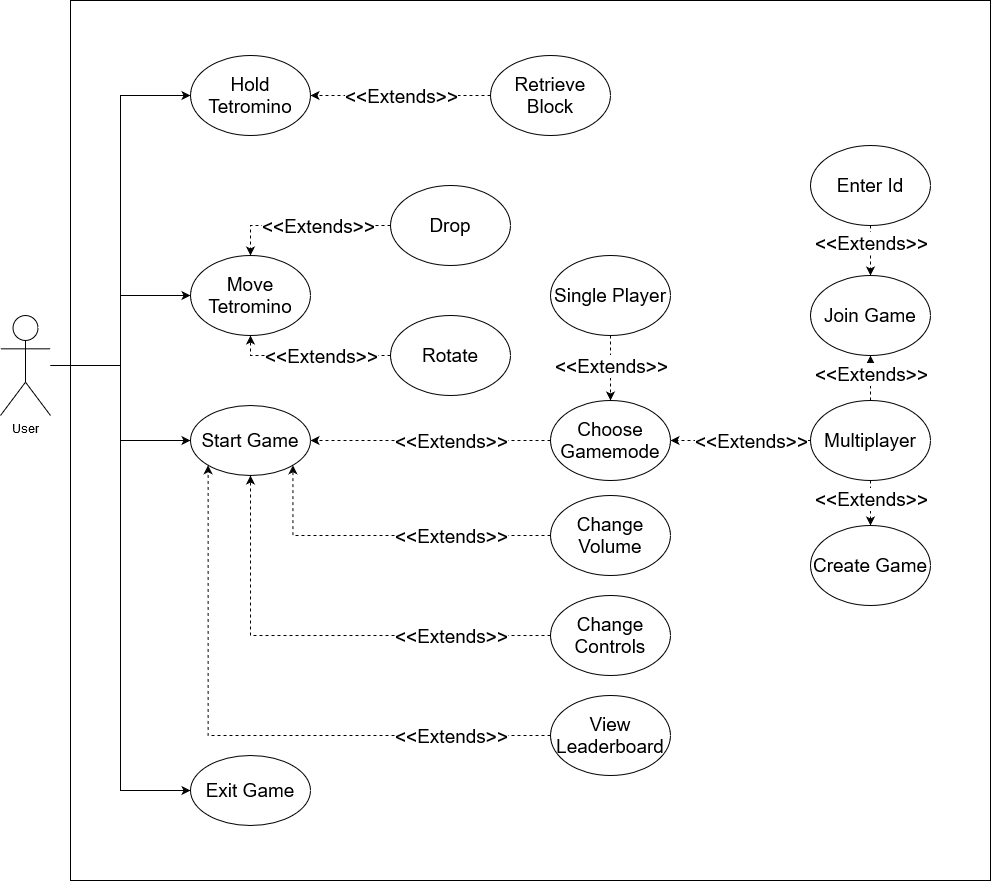
\includegraphics[width=5in]{usecase.png} 
    \caption{System Use Case Diagram}
    \label{wps}
\end{figure}

\begin{table}[H]
\caption{\bf Use Case 1: Hold Tetromino}
\begin{tabularx}{\textwidth}{|>{\raggedright\arraybackslash}p{3cm}|>{\raggedright\arraybackslash}X|}
\hline
\textbf{Use Case UC-1:} & \textbf{Hold Tetromino}  \\
\textbf{Related Requirements} & BE1: FR1 - FR3\\
&\\
\textbf{Initiating  Actor:} &  The user \\
&\\
\textbf{Actor's Goal:} & To hold an active Tetromino for later use\\
&\\
\textbf{Participating Actors:} & The user \\
&\\
\textbf{Preconditions:}  & The current active block was not held before\\
&\\
\textbf{Post conditions:}  & The current active block will be held\\
&\\
\textbf{Flow of Events for Main Success Scenario:} &\\
&\\
\textrightarrow & \textbf{1. User} has a current active block and presses the key to hold the block\\
&\\ 
& 2. \underline{extend::\textit{Retrieve Block}}\\
&\\
\textleftarrow & 3. \textbf{System} signals to the \textbf{user} the Tetromino has been held and switched the current active Tetromino\\
\hline
\end{tabularx}
\label{tab:UC-1}
\end{table}
\begin{table}[H]
\caption{\bf Use Case 4: View Leader Board}
\begin{tabularx}{\textwidth}{|>{\raggedright\arraybackslash}p{3cm}|>{\raggedright\arraybackslash}X|}
\hline
\textbf{Use Case UC-4:} & \textbf{View Leader Board}  \\
\hline
\textbf{Related Requirements} & BE4: FR1 - FR4\\
&\\
\textbf{Initiating  Actor:} &  The user \\
&\\
\textbf{Actor's Goal:} & To view the players with the highest scores\\
&\\
\textbf{Participating Actors:} & The user \\
&\\
\textbf{Preconditions:}  & The user is on the home or game screens\\
&\\
\textbf{Post conditions:}  & The leader board is shown to the user\\
&\\
\textbf{Flow of Events for Main Success Scenario:} &\\
&\\
\textrightarrow & \textbf{1. User} is on the home page or has completed a game and selects the view leader board option\\
&\\ 
\textleftarrow & 2.\textbf{System} signals to the \textbf{user} and displays the leader board\\
\hline
\end{tabularx}
\label{tab:UC-4}
\end{table}




\subsection{Functional Requirements}
\begin{enumerate}[{BE}1. ]

    \item The user wants to hold a Tetromino.
    \begin{enumerate}[{FR}1. ]
    \item The system shall provide the user with the ability to hold an active Tetromino.
    \item If there is a held Tetromino, the system must switch it with the current Tetromino.
    \item The user shall not be able to hold more than one Tetromino until the current Tetromino is placed.
    \end{enumerate}

    \item The user wants to move a Tetromino.
    \begin{enumerate}[{FR}1. ]
    \item The user shall be able to move an active Tetromino down, left, and right.
    \item The user must have the ability to rotate an active Tetromino 90\textdegree\ at a time.
    \item The user shall be able to rotate an active Tetromino clockwise and counterclockwise. 
    \item The system shall provide an option to drop an active Tetromino to the bottom of the screen.
    \item If an active Tetromino reaches the bottom of the board or a previously placed Tetromino, it becomes a dead Tetromino and must stop moving.
    \item Once a Tetromino is placed, the next Tetrimino shall become active and appear at the top of the board.
    \item After a Tetromino is placed, it must be unable to be moved by the player.
    \item If a line of Tetrominos is formed, that line will disappear and the remaining Tetrominos will move to the bottom of the board.
    \item If a line of Tetrominos is formed, the score must be updated.
    \item The scoring shall follow standard Tetris rules.\cite{tetris}
    \end{enumerate}
    
    \item The user wants to start the game.
    \begin{enumerate}[{FR}1. ]
    \item The system shall provide the user with multiplayer and single player options.
    \item The user shall be able to change the game's volume.
    \item There must be an option to change the controls of the game.
    \item The system shall provide an option to close the application.
    \item The system must generate Tetrominos randomly.
    \item The current Tetromino shall descend from the top of the board.
    \item The descending rate must increase as the game progresses.
    \item The next Tetromino shall be shown on screen.
    \item The game must end if there is a dead Tetromino with a portion above the board. 
    
    \end{enumerate}
    
    \item The user wants to view the leader board.
    \begin{enumerate}[{FR}1. ]
    \item The system shall provide the user with the ability to view the leader board from the home screen.
    \item The user shall be prompted with the ability to go to the leader board after completion of a game.
    \item The user must be able to scroll through the leader board rankings.
    \item The user shall be able to switch between the multiplayer and single player leader boards.
    \end{enumerate}

    \item The user wants to host a multiplayer game of Tetris.
    \begin{enumerate}[{FR}1. ]
    \item The system shall provide the user with the ability to create a multiplayer lobby.
    \item The system must provide a unique room code that another user can input to join the multiplayer lobby.
    \item The system must allow at most 2 people in a multiplayer lobby at a time.
    \end{enumerate}

    \item The user wants to join a multiplayer game of Tetris.
    \begin{enumerate}[{FR}1. ]
    \item The system shall provide the user with the ability to join a multiplayer lobby.
    \item The system will provide the user the ability to enter in a code to join the corresponding multiplayer lobby.
    \item The user must only be able to join one multiplayer lobby at a time.
    \end{enumerate}
    
\end{enumerate}
\section{Non-functional Requirements}

\subsection{Look and Feel Requirements}
\begin{enumerate}[{LFR}1. ]
    \item The games should look smooth with a consistent frame rate.
    \\\textbf{FIT CRITERION:} The game should run at a consistent 30 fps on the minimum recommended hardware.
    
    \item The game should include modern design elements and styling that reflect the visual trends in modern gaming.
    \\\textbf{FIT CRITERION:} A sample of 30 users that fit our game's demographic will complete a survey to indicate if they think the game looks modern.
    
    \item The text and game entities must be legible at a standard computer monitor viewing distance of 20-40 inches.\cite{OSHA}
    \\\textbf{FIT CRITERION:} A random sample of users will be tested to ensure the legibility of the game's visual elements.
    
    \item The typeface, iconography, and colouring must remain consistent throughout the system.
    \\\textbf{FIT CRITERION:} A sample of 30 users that fit our game's demographic will complete a survey to indicate if they think the game looks consistent.
\end{enumerate}

\subsection{Usability and Humanity Requirements}
\begin{enumerate}[{UHR}1. ]
    \item Mechanisms will be in place to instruct the user of what to do in specific areas of the game.
    \\\textbf{FIT CRITERION:} 90\% of users must be able to play the main game after reading the instructions.
    
    \item System will follow the correct colour contrast ratio(s) for text and backgrounds to make the visual elements of the game legible to users.
    \\\textbf{FIT CRITERION:} All colour contrast ratio's will be within the range dictated by the Web Content Accessibility Guidelines \cite{contrast}
    
    \item All buttons necessary for user interaction must be easily identifiable on screen.
    \\\textbf{FIT CRITERION:} Sample users must be able to locate and press selected buttons on the screen within 5 seconds.
    
    \item The language should be easily understood by users.
    \\\textbf{FIT CRITERION:} Sample users with at least a fifth grade reading comprehension level can comprehend all the text in the game.
\end{enumerate}

\subsection{Performance Requirements}
\begin{enumerate}[{PR}1. ]
    \item The game must be responsive to valid users inputs. 
    \\\textbf{FIT CRITERION:} The average response time between user input and game response should be less than 0.25 seconds.
    
    \item The system should support at least 40 users concurrently.
    \\\textbf{FIT CRITERION:} The system is still able to run without crashing while 40 instances of the game are running concurrently on different machines. 
    
    \item The system shall quickly respond to network requests with the necessary information.
    \\\textbf{FIT CRITERION:} The system shall respond in less than 3 seconds 99\% of the time.
    
    \item The system shall have an availability of at least 99.99\%.
    \\\textbf{FIT CRITERION:} The system's downtime will be measured to ensure high availability.
    
	\item The system shall require internet access for multiplayer functionality.
	\\\textbf{FIT CRITERION:} The system will be tested on machines on separate networks.

\end{enumerate}

\subsection{Operational and Environmental Requirements}
\begin{enumerate}[{OER}1. ]
    \item The game will be able to run on browsers installed on systems with an operating system of Windows 10, Mac OSX or Linux.
    \\\textbf{FIT CRITERION:} The game will be run on all three operating systems without crashing. 
    
    \item The game will be able to run on different modern browsers with HTML5 and JavaScript enabled.
    \\\textbf{FIT CRITERION:} The game will be run on a set of browsers with HTML5 and JavaScript compatibility without crashing. 
\end{enumerate}

\subsection{Maintainability and Support Requirements}
\begin{enumerate}[{MSR}1. ]
    \item System updates shall not keep the system down for longer than 10 minutes.
    \\\textbf{FIT CRITERION:} A timer will be used to check for adherence to this limit. 
    \item The software will be supported by the developers for a minimum of one year.
    \\\textbf{FIT CRITERION:} Every month a patch will be released to the system, fixing any reported bugs.
\end{enumerate}
\subsection{Security Requirements}
\begin{enumerate}[{SR}1. ]
    \item The system source code shall only be modified by the developers of the system.
    \\\textbf{FIT CRITERION:} All modifications of source code will be managed through Gitlab, allowing only the development team to make code changes.
    \item The system shall enforce an encrypted connection between users and the server.
    \\\textbf{FIT CRITERION:} Connection between users and the server will be done using Hypertext Transfer Protocol Secure (HTTPS).
\end{enumerate}
\subsection{Cultural Requirements}
\begin{enumerate}[{CR}1. ]
    \item The iconography and language will be inoffensive to as many users as possible.
    \\\textbf{FIT CRITERION:} The system shall not contain any hate symbols defined by the Anti Defamation League (ADL). \cite{adl}
\end{enumerate}
\subsection{Legal Requirements}
\begin{enumerate}[{LR}1. ]
    \item The system must obey applicable laws and regulations.
    \\\textbf{FIT CRITERION:} The system will obey Canadian federal laws, Ontario's provincial laws, and Hamilton's municipal by-laws.
\end{enumerate}
\subsection{Health and Safety Requirements}
\begin{enumerate}[{HSR}1. ]
    \item The system must not cause the users any adverse health effects related to prolonged play or use from a game session.
    \\\textbf{FIT CRITERION:} The total in game play time of any game session will not exceed 60 minutes.
    \item The system will not cause exposure to undo epileptic risks.
    \\\textbf{FIT CRITERION:} The system will conform with the guidelines set out by WCAG. \cite{wcag}
\end{enumerate}
\section{Project Issues}
\subsection{Open Issues}
\begin{enumerate}[{Issue }1.]
\item Currently, it is not decided on how to fully implement the multiplayer component and that could have a significant impact on the user experience. 
\end{enumerate}

\subsection{Off-the-Shelf Solutions}
Currently there are many options for playing Tetris online and on mobile devices. Examples such as \url{https://tetris.com/play-tetris} along with numerous knockoffs offer similar product experiences and features. Features such as: user interface and menu, multiplayer, and scoring and leader boards. However although the products are similar, no other product we found gave the user the option to hold a Tetromino along with the rest of the features.

\subsection{New Problems}
No new problems.
\subsection{Tasks}
\begin{enumerate}
    \item Create game menu
    \item Create game interface
    \item Create game model 
    \item Create multiplayer mode
    \item Create leader board and scoring system
    \item Proof of concept testing and demonstration
    \item Conduct first code revision
    \item Further Tasks to be posted at revision
\end{enumerate}

\subsection{Migration to the New Product}
Not applicable.
\subsection{Risks}
The only current major risk is related to our lack of experience as developers with and implementing a multiplayer game feature. We will be mitigating this, by beginning to work on that aspect immediately so we have additional time to deal with unforeseen issues. Other implementation risks are considered less relevant as there are many examples of similar working products.
\subsection{Costs}
The development of this system will have no cost since all libraries and pieces of source code that will be used are open source. 
\subsection{User Documentation and Training}
The system will be run as a web application that can be found through an internet browser that is HTML5 compatible. There will be no documentation for this section as we assume the user knows how to operate and navigate a web browser. There will be a section integrated within the game to teach the user how to play Tetris.


\subsection{Waiting Room}
Features to be considered for future releases:
\begin{enumerate}
    \item Interchangable UI skins
    \item In-game chat
    \item User accounts to hold statistics
    \item Audio/music
    \item AI opponent
\end{enumerate}

\subsection{Ideas for Solutions}
A possible solution for issue 1 the multiplayer component: is to use web sockets and JavaScript to facilitate the communication between the game clients.
\newpage
\section{Appendix}
\subsection{Symbolic Parameters}
N/A
\subsection{References}
\bibliography{references}
\end{document}